\documentclass[14pt,a4paper]{extarticle}

\usepackage{fontspec}
\setmainfont{Times New Roman}
\setsansfont{Arial}
\setmonofont{Courier New}[Scale=MatchLowercase]

\usepackage[
  a4paper,
  left=25mm,
  right=20mm,
  top=20mm,
  bottom=20mm,
  headheight=17pt,
  headsep=7mm,
  footskip=10mm
]{geometry}

\usepackage{setspace}
\setstretch{1.5}
\usepackage{indentfirst}
\setlength{\parindent}{1.25cm}
\setlength{\emergencystretch}{3em}

\usepackage[russian,english]{babel}
\usepackage{csquotes}
\usepackage{xcolor}
\usepackage{xurl}
\usepackage{pdfpages}
\usepackage{enumitem}
\usepackage{array}
\urlstyle{same}

\usepackage[
  colorlinks=true,
  linkcolor=black,
  citecolor=black,
  urlcolor=black
]{hyperref}

\usepackage{fancyhdr}
\pagestyle{fancy}
\fancyhf{}
\fancyhead[R]{\thepage}
\renewcommand{\headrulewidth}{0pt}

\sloppy

\begin{document}
\selectlanguage{russian}

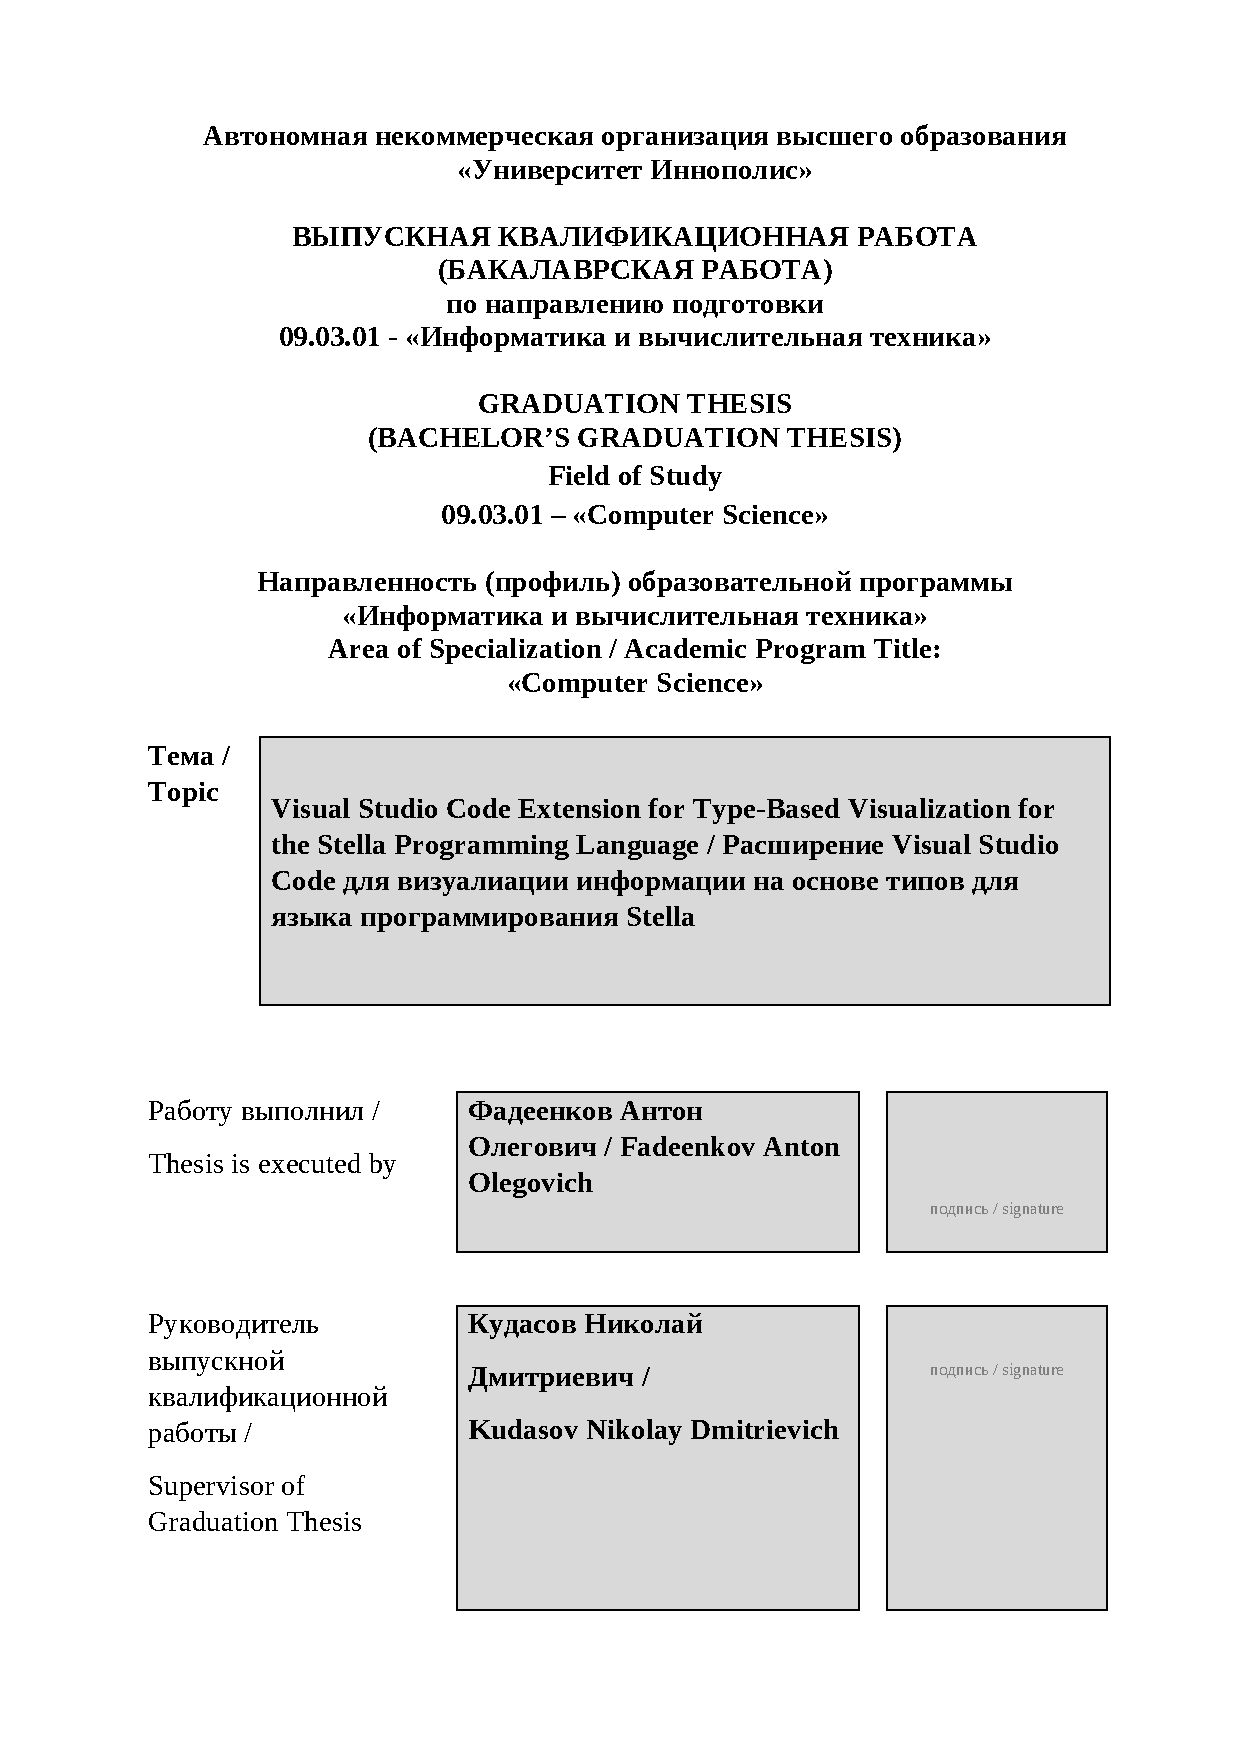
\includepdf[pages=1, pagecommand={\thispagestyle{empty}}]{title.pdf}
\setcounter{page}{2}

\section*{Введение, цель и задачи}

Выпускная квалификационная работа посвящена разработке расширения Visual Studio Code для визуализации результатов синтаксического и типового анализа программ на языке Stella. Stella является учебным статически типизированным языком, который используется при изучении систем типов и принципов построения компиляторов. Для таких курсов важно видеть не только итоговую ошибку или выведенный тип, но и промежуточные структуры анализа: абстрактное синтаксическое дерево, контекст типизации, дерево вывода типов и зависимости между выражениями.

Проблема состоит в том, что стандартные средства редактора обычно показывают только конечный результат работы языкового сервера: подсказку, подчеркивание ошибки или краткое диагностическое сообщение. В результате студенту приходится самостоятельно восстанавливать, какие подвыражения участвовали в проверке и почему было получено суждение $\Gamma \vdash e : T$, где $\Gamma$ обозначает контекст типизации, $e$ --- выражение, а $T$ --- его тип.

Цель работы --- спроектировать и реализовать расширение Visual Studio Code, которое представляет результаты анализа Stella в виде интерактивных представлений, связанных с исходным кодом. Для достижения цели были изучены подходы к образовательной визуализации, определены необходимые представления, спроектирован обмен данными между клиентом и языковым сервером, реализованы пользовательские запросы Language Server Protocol и проведена функциональная проверка прототипа.

\section*{Обзор литературы}

Визуализация программ применяется в обучении информатике для объяснения структур и процессов, которые трудно наблюдать напрямую. Работы по software visualization и algorithm visualization показывают, что интерактивные представления могут поддерживать понимание абстрактных процессов, однако их результаты нельзя автоматически переносить на конкретный инструмент без отдельной проверки. Поэтому исследования Price, Hundhausen, Naps, Sorva и Kogan используются в работе как основание для проектирования, а не как прямое доказательство эффективности расширения.

Близкими по тематике являются Jeliot и visAST. Jeliot визуализирует выполнение программ, а visAST связывает исходный текст с абстрактным синтаксическим деревом. Отличие данной работы состоит в том, что разработанное расширение охватывает не только синтаксис, но и информацию, связанную с типами: контекст типизации, дерево вывода, трассу ошибки и граф зависимостей. Теоретическую основу составляют работы по статическим системам типов, суждениям типизации и анализу программ.

\section*{Краткое описание основного содержания работы}

В работе разработан прототип расширения Visual Studio Code для языка Stella. Клиентская часть реализует пользовательские представления редактора, а серверная часть подготавливает данные анализа и передает их через расширенные запросы Language Server Protocol. Для обмена используется JSON-RPC, что согласуется с архитектурой LSP и позволяет отделить вычисление результатов анализа от их отображения в интерфейсе.

Основными результатами являются пять представлений. AST View показывает структуру программы в виде дерева. Scope View отображает область видимости и контекст типизации. Type Derivation View показывает последовательность применения правил вывода типов. Type Error Trace View помогает проследить путь к ошибке типизации. Type Dependency Graph показывает зависимости между выражениями и типовыми суждениями; такое представление связано с идеями program dependence graph и program slicing, но адаптировано к учебному языку Stella.

Отдельное внимание уделено согласованию технологического стека с принципами проектирования. TypeScript выбран как основной язык реализации из-за строгой типизации и совместимости с экосистемой Visual Studio Code. Langium используется для реализации языковой инфраструктуры, а API Visual Studio Code --- для построения Tree View и Webview-представлений. Такой стек позволяет сохранить связь между анализом, редактором и пользовательским интерфейсом без отдельного внешнего приложения.

Проверка результата выполнена функционально: были рассмотрены типовые программы Stella, корректность ответов языкового сервера и отображение результатов в интерфейсе редактора. Полноценное пользовательское исследование не проводилось, поэтому выводы об удобстве и влиянии на понимание ограничены. Это ограничение явно учитывается как угроза корректности результатов.

\section*{Заключение}

В результате работы было создано расширение Visual Studio Code, которое визуализирует промежуточные результаты анализа программ на языке Stella. Расширение показывает не только итоговый результат проверки, но и структуры, которые участвуют в синтаксическом и типовом анализе. Это делает прототип полезным как вспомогательный инструмент для изучения реализации систем типов.

Основной вклад работы состоит в проектировании набора представлений для Stella, реализации обмена данными между расширением и языковым сервером, создании пользовательского интерфейса в Visual Studio Code и функциональной проверке прототипа. Дальнейшее развитие работы может включать полноценное пользовательское исследование, оценку удобства по SUS, улучшение визуализации графов и расширение поддержки новых конструкций языка Stella.
\section*{Список использованных источников}

\begin{enumerate}[label={[\arabic*]},leftmargin=*,itemsep=0pt,topsep=0pt]
\item Microsoft. Language Server Protocol Specification 3.17. URL: \url{https://microsoft.github.io/language-server-protocol/specifications/lsp/3.17/specification/}.
\item JSON-RPC Working Group. JSON-RPC 2.0 Specification. URL: \url{https://www.jsonrpc.org/specification}.
\item Microsoft. Visual Studio Code Extension API. URL: \url{https://code.visualstudio.com/api}.
\item Microsoft. Visual Studio Code Tree View API. URL: \url{https://code.visualstudio.com/api/extension-guides/tree-view}.
\item Microsoft. Visual Studio Code Webview API. URL: \url{https://code.visualstudio.com/api/extension-guides/webview}.
\item TypeFox. Langium Documentation. URL: \url{https://langium.org/docs/}.
\item Kudasov N. Stella Language Documentation. URL: \url{https://fizruk.github.io/stella/site/core/introduction/}.
\item Abounegm A., Kudasov N., Stepanov A. Teaching Type Systems Implementation with STELLA. 2024. URL: \url{https://arxiv.org/abs/2407.08089}.
\item Pierce B. C. Types and Programming Languages. MIT Press, 2002.
\item Harper R. Practical Foundations for Programming Languages. Cambridge University Press, 2016.
\item Nielson F., Nielson H. R., Hankin C. Principles of Program Analysis. Springer, 1999.
\item Price B. A., Baecker R. M., Small I. S. A Principled Taxonomy of Software Visualization // Journal of Visual Languages and Computing. 1993.
\item Hundhausen C. D., Douglas S. A., Stasko J. T. A Meta-Study of Algorithm Visualization Effectiveness // Journal of Visual Languages and Computing. 2002.
\item Naps T. L. et al. Exploring the Role of Visualization and Engagement in Computer Science Education // ITiCSE Working Group Reports. 2002.
\item Sorva J., Karavirta V., Malmi L. A Review of Generic Program Visualization Systems // ACM Transactions on Computing Education. 2013.
\item Moreno A., Myller N., Sutinen E., Ben-Ari M. Visualizing Programs with Jeliot 3 // AVI. 2004.
\item Aalvik R. visAST: Generic AST Visualiser for Software Language Education: master's thesis. University of Bergen, 2019.
\item Ferrante J., Ottenstein K. J., Warren J. D. The Program Dependence Graph and Its Use in Optimization // ACM TOPLAS. 1987.
\item Brooke J. SUS: A Quick and Dirty Usability Scale // Usability Evaluation in Industry. Taylor \& Francis, 1996.
\item Bangor A., Kortum P., Miller J. Determining What Individual SUS Scores Mean // Journal of Usability Studies. 2009.
\item Wohlin C. et al. Experimentation in Software Engineering. Springer, 2012.
\item Runeson P., Hoest M. Guidelines for Conducting and Reporting Case Study Research in Software Engineering // Empirical Software Engineering. 2009.
\end{enumerate}

\end{document}








